\section{Exercises}
\begin{exercise}[\textbf{Counting}]
Given an integer number $X$, we would like to count in how many ways it can be represented as a sum of $N$ natural numbers (with relevance to order) marked by ${\Psi _N}\left( X \right)$. For example, ${\Psi _2}\left( 3 \right) = 2$ since: $3 = 1 + 2 = 2 + 1$.
\begin{enumerate}
  \item Find the following: ${\Psi _1}\left( 2 \right),{\Psi _2}\left( 4 \right),{\Psi _3}\left( 2 \right),{\Psi _N}\left( N \right)$ and ${\Psi _1}\left( X \right)$.
  \item Find a recursive equation for ${\Psi _N}\left( X \right)$.
  \item Write a code in Matlab for finding ${\Psi _N}\left( X \right)$ using dynamic programming.
  \begin{enumerate}
    \item What is the time and memory complexity of your algorithm?
    \item Find ${\Psi _{12}}\left( {800} \right)$.
  \end{enumerate}
  \item Now assume each natural number $i$ is associated with some cost ${c_i}$. For a given $X,N$ we are interested in finding the lowest cost combination of natural numbers $\left\{ {{x_i}} \right\}_{i = 1}^N$ satisfying $\sum\nolimits_{i = 1}^N {{x_i}}  = X$.
      \begin{enumerate}
        \item Formulate the problem as a finite horizon decision problem: Define the state space, the action space and the cumulative cost function.
        \item Bound the complexity of finding the best combination.
      \end{enumerate}
\end{enumerate}
\end{exercise}

\begin{exercise}[\textbf{Language model}]
In the city of Bokoboko the locals use a language with only 3 letters ('B','K','O'). After careful inspection of this language, researchers have reached two conclusions:
\begin{itemize}
  \item[I.]	Every word starts with the letter 'B'.
  \item[II.] Every consecutive letter is distributed only according to the previous letter as follows:
\[P\left( {{l_{t + 1}}|{l_t}} \right) = \begin{array}{*{20}{c}}
B\\
K\\
O\\
 -
\end{array}\left[ {\begin{array}{*{20}{c}}
{0.1}&{0.325}&{0.25}&{0.325}\\
{0.4}&0&{0.4}&{0.2}\\
{0.2}&{0.2}&{0.2}&{0.4}\\
1&0&0&0
\end{array}} \right]\]
Where '-' represents the end of a word. For example, the probability of the word 'bko' is given by $0.325 \cdot 0.4 \cdot 0.4 = 0.052$.
\end{itemize}

\begin{enumerate}
  \item Find the probability of the following words: 'Bob', 'Koko', 'B', 'Bokk','Boooo'.
  \item We wish to find the most probable word in the language of length $K$.
\begin{enumerate}
  \item Formulate the problem as a finite horizon decision problem: Define the state space, the action space and the multiplicative cost function.
  \item Bound the complexity of finding the best combination.
  \item Find a reduction from the given problem to an analogous problem with additive cost function instead.
  \item Explain when each approach (multiplicative vs. additive) is preferable. \\Hint: Think of the consequence of applying the reduction on the memory representation of a number in a standard operating system.
  \item Write a code in Matlab which finds the most probable word of a given size using dynamic programming. What is the most probable word of size 5?
\end{enumerate}
\end{enumerate}
\end{exercise}

\begin{exercise}[Path Planning]
Moses the mouse starts his journey at the south west room in a $M \times N$ rectangular apartment with $M \cdot N$ rooms of size $1 \times 1$, some of which contain cheese. After his rare head injury in the mid-scroll war, Moses can only travel north or east. An illustration of Moses's life for $M = 5,N = 8$ is given in the following figure.

\begin{center}
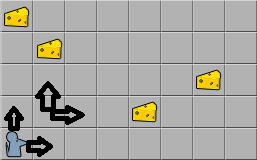
\includegraphics[width=0.5\textwidth]{hw1_a}
\end{center}

Being a mouse and all, Moses wants to gather as much cheese as possible until he reaches the north-east room of the apartment.
\begin{enumerate}
  \item Formulate the problem as a finite horizon decision problem: Define the state space, the action space and the cumulative cost function.
  \item What is the horizon of the problem?
  \item How many possible trajectories are there? How does the number of trajectories behaves as a function of $N$ when $M = 2$? How does it behave as a function of $N$  when $M = N$?
  \item Aharon, Moses's long lost war-buddy woke up confused next to Moses and decided to join him in his quest (needless to say, both mice suffer the same rare head injury).
      \begin{enumerate}
        \item Explain what will happen if both mice ignore each other's existence and act 'optimal' with respect to the original problem.
        \item Assume both mice decided to coordinate their efforts and split the loot. How many states and actions are there now?
        \item Now their entire rarely-head-injured division has joined the journey. Assume there's a total of $K$ mice, how many states and actions are there now?
      \end{enumerate}
\end{enumerate}
\end{exercise}

\begin{exercise}[\textbf{MinMax dynamic programming}]
In this problem we consider an adversarial version of finite horizon dynamic programming, which is suitable for solving 2-player games. 

In this setting, at time $k \in \left\{ {0,1,2, \ldots ,N - 1} \right\}$ the system is at state ${s_k} \in {S_k}$, the agent chooses an action ${a_k} \in {A_k}\left( {{s_k}} \right)$ according to the agent policy $\pi _k^a({s_k})$, and subsequently the opponent chooses an action ${b_k}$ from the set of allowable opponent actions ${B_k}\left( {{s_k},{a_k}} \right)$, according to the opponent policy $\pi _k^b({s_k},{a_k})$.

The system then transitions to a new state according to:
$${s_{k + 1}} = {f_k}({s_k},{a_k},{b_k}),\quad k = 0,1,2, \ldots ,N - 1.$$
The instantaneous reward is denoted by $r\left( {{s_k},{a_k},{b_k}} \right)$, and, for an N-stage path ${h_N} = ({s_0},{a_0},{b_0} \ldots ,{s_{N - 1}},{a_{N - 1}},{b_{N - 1}},{s_N})$ the cumulative reward is
$${R_N}({h_N}) = \sum\limits_{k = 0}^{N - 1} {{r_k}({s_k},{a_k},{b_k}) + {r_N}({s_N})} .$$
Given ${s_0}$, the agent's goal is to find a policy $\pi _a^*$ that maximizes the worst-case cumulative reward:
$$\pi _a^* \in \argmax_{\pi_a} \left\{ {\min_{\pi_b}} \left\{{R_N}({h_N})\right\}\right\}.$$
\begin{enumerate}
  \item Formulate a dynamic programming algorithm for this problem. Explain what the value function represents in this case.
  \item What is the computational complexity of your algorithm?
  \item Could this approach be used to solve the game of tic-tac-toe? Explain what are the states, actions and rewards for this game.
  \item Could this approach be used to solve the game of chess? Explain.
\end{enumerate}
\end{exercise}

\begin{exercise}[\textbf{SSSP}]This exercise concerns the SSSP problem.

\begin{enumerate}
  \item Give an example of a graph that does not contain negative cycles, but for which Dijkstra's algorithm fails. Prove that your graph indeed does not contain any negative cycles.
  \item Consider the following road distances table (Excel file available on the course web-page). Each number in the table represents a road between the two cities of the mentioned distance.
\begin{table}[]
\centering
\resizebox{\textwidth}{!}{%
\begin{tabular}{lllllllllll}
 & Eilat & Ashdod & Beer Sheva & Haifa & Jerusalem & Nazereth & Netanya & Petah Tikva & Rehovot & Tel Aviv \\
Eilat & 0 & 328 & 246 & - & 323 & - & 381 & - & 327 & - \\
Ashdod & 328 & 0 & 82 & - & - & - & - & 47 & 24 & 42 \\
Beer Sheva & 246 & 82 & 0 & - & 89 & - & - & 106 & 82 & 103 \\
Haifa & - & - & - & 0 & 145 & 40 & 64 & 91 &  & 95 \\
Jerusalem & 323 & - & 89 & 145 & 0 & 142 & - & 60 & 59 & 62 \\
Nazereth & - & - & - & 40 & 142 & 0 & 75 & - & - & - \\
Netanya & 381 & - & - & 64 & - & 75 & 0 & 30 & 54 & 33 \\
Petah Tikva & - & 47 & 106 & 91 & 60 & - & 30 & 0 & 29 & 10 \\
Rehovot & 327 & 24 & 82 & - & 59 & - & 54 & 29 & 0 & 21 \\
Tel Aviv & - & 42 & 103 & 95 & 62 & - & 33 & 10 & 21 & 0
\end{tabular}
}
\caption{City-distances}
\end{table}
  \begin{enumerate}
    \item How many nodes and edges are there in the induced graph?
    \item What is the shortest path between Tel Aviv and Haifa? What about Jerusalem and Nazereth?
    \item Program Dijkstra's algorithm and find the shortest path from each city to each other city. What is the time complexity of your solution in terms of the number of nodes and edges in the graph?
    \item Find the shortest route that starts at Jerusalem, visits all other cities and then returns to Jerusalem. What is the time complexity of your solution in terms of the number of nodes and edges in the graph?
  \end{enumerate}
\end{enumerate}
\end{exercise}